\chapter{Introducción}
\label{cap:introduccion}

En los últimos años, el aumento en el tamaño y la complejidad en los videojuegos ha supuesto la imprescindible optimización y automatización de diversos aspectos de su desarrollo, tanto en el ámbito del renderizado como en la lógica interna de los sistemas. Particularmente la evolución de entornos 3D, con el objetivo de obtener gráficos más detallados, ha implicado un incremento significativo en el coste computacional. Una forma de afrontar estas simulaciones para reducir su impacto computacional, es utilizar modelos de ML que permiten aproximar el comportamiento de estos elementos reduciendo el coste.\newline

Empresas pioneras en hardware y software han desarrollado tecnologías para mejorar el rendimiento gráfico incorporando esta clase de algoritmos. Entre ellas destacan: NVIDIA con DLSS (Deep Learning Super Sampling), que se ha utilizado en multitud de videjuegos como por ejemplo el Resident Evil Requiem que usa DLSS 4\footnote{ \textbf{\href{https://www.nvidia.com/es-la/geforce/news/dlss-4-rtx-path-tracing-game-announcements-ces-2026/}{Deep Learning Super Sampling:}} aumenta el rendimiento del videojuego permitiendolo renderizarse con una resolución más baja, ya que esta tecnología consigue reconstruir la imagen a mayor calidad en runtime. Utiliza herramientas como \textit{Ray Reconstruction} para reemplazar sus \textit{denoisers} manuales o DLAA (Deep Learning Anti-Aliasing) para suavizar los bordes.}; y AMD con FSR4 (FidelityFX Super Resolution)\footnote{ \textbf{\href{https://www.amd.com/en/products/graphics/technologies/fidelityfx/super-resolution.html}{FidelityFX Super Resolution Upscaling:}} técnica desarrollada por AMD de código abierto que consiste en el aumento del rendimiento en videojuegos mediante el escalado de resolución. Se diferencia del DLSS de NVIDIA por tener requerimientos menos específicos de hardware, así como efectos visuales más suaves.}. Asimismo, varias compañías lo incorporan en la lógica del juego simulando comportamientos y mecánicas como EA (FIFA \footnote{\textbf{\href{https://news.ea.com/press-releases/press-releases-details/2021/EA-SPORTS-Introduces-FIFA-22-With-Next-Gen-HyperMotion-Technology-Bringing-Footballs-Most-Realistic-and-Immersive-Gameplay-Experience-to-Life/default.aspx}{HyperMotion}:} introducida en el FIFA22, es una tecnología que combina captura de movimiento y aprendizaje automático para generar nuevas animaciones a tiempo real y crear un movimiento orgánico y fluido en el juego}), Embark Studios (Arc Raiders \footnote{\textbf{\href{https://schedule.gdconf.com/session/learning-to-move-physics-based-enemy-locomotion-in-arc-raiders/917319}{Physics-Based Enemy Locomotion:}} crea los movimientos del enemigo basándose en aprendizaje por refuerzo, combinando físicas, conceptos de robótica y aportando enemigos con capacidad de decisión sobre sus movimientos.}) o Ubisoft con sus múltiples lineas de investigación sobre la IA. En este contexto, un tercer campo de aplicación que está en proceso de investigación es la aplicación de modelos de aprendizaje automático en simulaciones físicas. \newline

En el campo de la simulación física, con el incremento de la capacidad de cálculo de los sistemas actuales, se busca una mayor fidelidad en la recreación de las interacciones entre los diferentes elementos. Así por ejemplo, elementos como el cabello, los fluidos o las telas, elementos que hace poco más de una década estaban muy simplificados, en la actualidad se busca cada vez más con comportamiento realista en sus interacciones. Esta simulación física de sus comportamientos resulta en una carga computacional significativa, lo que afecta negativamente al rendimiento de los videojuegos, en especial en términos de tasa de fotogramas. La industria se encuentra en un momento de auge en investigación y aplicación de Machine Learning para solucionarlo. Se puede observar por ejemplo, a través de los estudios de Ubisoft la Forge, el grupo de desarollo e investigación de Ubisoft\footnote{Artículos y publicaciones de Ubisoft la Forge: \url{https://www.ubisoft.com/en-us/studio/laforge/publications\#24A8zwsBgQ1tTMlNRp20b9\%C3\%A7}}. Entre sus investigaciones se encuentran aplicaciones recientes de ML en distintos campos de simulación; la adaptación de animaciones de personajes a interacciones físicas \cite{drecon2019} o la aceleración de simulaciones de cuerpos deformables \cite{holden_subspace_2019}, sobre el que se profundizará en el siguiente capítulo. \newline



\section{Motivación}
En la misma línea de otras tecnologías ya utilizadas en el desarrollo de videojuegos como la mencionada DLSS de NVDIA, donde se aplican modelos de redes neuronales profundas para reducir la carga computacional de los juegos en el renderizado, se conducen estudios y empiezan a aplicar técnicas similares en la industria en simulación física. Nace en un contexto donde los juegos tienden a ser distribuidos ya no solo en consolas con hardware y gráficas dedicadas, sino en múltiples plataformas con el objeto de maximizar ingresos, donde no todas tienen las mismas capacidades de cómputo.  El uso de estas técnicas de optimización puede permitir recrear estas simulaciones con un grado de fidelidad aceptable, en dispositivos de menor potencia como pueden ser Nintendo Switch, Handle pcs o dispositivos móviles. Así mismo, en cada vez en más dispositivos, incluso de bajo rendimiento (en comparación con consolas de sobremesa o PC preparados para juegos) se incluyen algún tipo de hardware de aceleración de redes neuronales, como por ejemplo la propia Nintendo Switch 2 que dispone de 48 tensor cores o Xbox rog ally X con una NPU AMD XDNA lo que nos abre un abanico de posibilidades para ejecutar estos modelos de forma más eficiente.\newline

La motivación principal de este estudio reside en lograr simulaciones visualmente verosímiles, que se centren en la percepción del usuario. Por ello, se ha optado por la simulación de telas. La simulación de telas se presenta como un caso de físicas complejas, alto dinamismo y aplicación tanto en optimización en juegos integrados como en herramientas para artistas, ofreciendo un amplio rango de usos, que comienza a integrarse a día de hoy en grandes empresas y continua en fase experimental. Se elige este caso de uso pues representa un equilibrio adecuado entre complejidad física y familiaridad con el resultado visual, que permite llevar a cabo un análisis tanto técnico como perceptivo.

\section{Objetivos}
El objetivo general de este proyecto es construir una infraestructura que permita identificar las limitaciones actuales de la implementación de un modelo de IA que replique el movimiento en tiempo real de una tela en un motor de videojuegos con baja latencia. Para cumplir con este objetivo, se plantean las siguientes metas durante el desarrollo del proyecto:

\begin{enumerate}
	%\renewcommand{\theenumi}{\alph{enumi}}
	\item Generar una animación de una tela y un colisionador que varíe su movimiento en cada ejecución de la escena.
	\item Generar y procesar datasets con la información relevante de la tela respecto a su entorno y colisionador.
	\item Implementar, entrenar y evaluar los distintos modelos de aprendizaje automático, tales como redes neuronales.
	\item Analizar y comparar los resultados tanto visuales como de rendimiento de los distintos modelos.
\end{enumerate}

\section{Plan de trabajo}
El desarrollo del proyecto se llevará a cabo en el perido lectivo del curso 2025-2026. Dados los objetivos del apartado anterior, la planificación se divide en las siguientes iteraciones:

\begin{itemize}
\item \textbf{Iteración 0:} En esta etapa se concretan los objetivos reales de la investigación y se establece la planificación del trabajo respecto a la propuesta inicial.

\item \textbf{Iteración 1:} Etapa de preparación, donde se cumplirán los siguientes subobjetivos para implementar un sistema de simulación adecuado para ser procesado por los modelos en un futuro.
	\begin{itemize}
        \item \textbf{Iteración 1.1:} Se realizará una investigación de trabajos relacionados a este, relevante para dirigir el desarrollo de los experimentos. Se analizarán distintas alternativas y se decidirá cuales resultarán más interesantes de replicar, se definirán qué tipo de datos deberemos recopilar para el entrenamiento y qué tipo de redes podrán llevarlo a cabo.
   		\item \textbf{Iteración 1.2:} Se creará una simulación básica en Unity y un sistema de registro de datos relevantes a la tela.
   	\end{itemize}
\item \textbf{Iteración 2:} Se establecerá un entorno de trabajo para el entrenamiento de los datos recopilados. Se generará un pipeline claro en el que se integre la simulación de recogida de datos, su limpieza y posterior uso para entrenar el modelo y, finalmente, la incorporación de este al entorno de simulación. Para poder asegurar del correcto funcionamiento de este sistema se generará un modelo simple y se comprobará que el pipeline es correcto. En esta fase se comenzarán a redactar los primeros capítulos de la memoria.

\item \textbf{Iteración 3:} Con una base sólida ya montada, se aumentará la complejidad y, por consiguiente, el coste de la simulación. Se implementarán distintos modelos y se llevarán a cabo pruebas con todos ellos para asegurarse de su fiabilidad.

\item \textbf{Iteración 4:} Si las anteriores iteraciones funcionan de manera correcta esta última no tendrá ninguna carga de implementación. Se alcanzará la última meta definida: hacer distintas pruebas entrenando los modelos ya desarrollados, sacar métricas de todos ellos para poder hacer comparaciones y hacer un análisis exhaustivo de estos resultados, sacando así las conclusiones de la investigación.
\end{itemize}

El desarrollo de las tareas y su planificación se puede ver en la figura \ref{fig:diagrama-gantt}.
\begin{figure}[H]
	\centering
	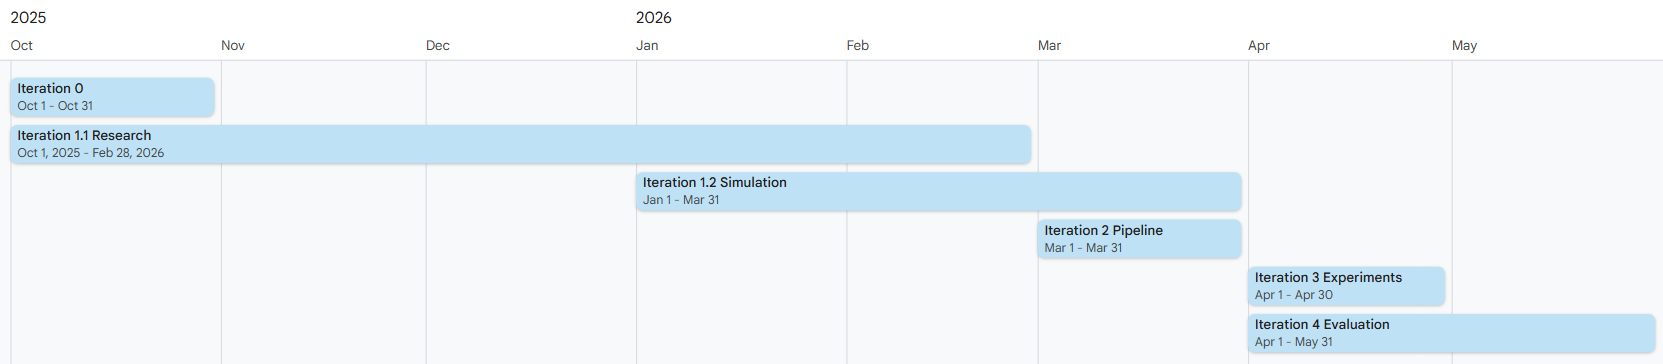
\includegraphics[width=0.91\textwidth]{Imagenes/GanntChart.png}
	\caption{Diagrama de Gantt del proyecto. Representa la organización de las tareas en el tiempo de desarrollo del proyecto.}
	\label{fig:diagrama-gantt}
\end{figure}

\section{Entorno de trabajo}
Para el desarrollo de esta investigación se emplearán herramientas de libre acceso y uso gratuito, con el objetivo de facilitar la reproducibilidad de los resultados obtenidos. El entorno de desarrollo principal será Windows 11, al tratarse del sistema operativo utilizado por el equipo de trabajo y extendido entre los potenciales usuarios. La simulación de la tela, así como la integración del modelo de inteligencia artificial, se llevarán a cabo en Unity (versión 6000.3.2f1, correspondiente a una versión de soporte a largo plazo). En cuanto a los lenguajes de programación, se empleará C\# para el desarrollo dentro de Unity, incluyendo la generación de la simulación y la recopilación de datos, mientras que se utilizará Python con Pytorch para el entrenamiento de los modelos de aprendizaje automático. La integración de los modelos entrenados en el entorno de ejecución se realizará a traves del paquete Unity Sentis.

Para la gestión del código fuente y el trabajo colaborativo se utilizará GitHub, basado en el sistema de control de versiones Git. Asimismo, se empleará la herramienta GitHub Projects para la planificación, asignación y seguimiento de tareas. Como herramientas adicionales, se utilizará Google Drive para el almacenamiento de documentación, apuntes de reuniones y materiales de trabajo puntuales, y Discord para la coordinación del equipo mediante reuniones online, además de encuentros presenciales semanales.

%+\section{Estructura de la memoria (propuesta)}